\documentclass[french,a4paper,10pt,twocolumn]{article}
\usepackage{graphicx} % Required for inserting images
\usepackage[style=authoryear, backend=biber]{biblatex}
\usepackage[left=1cm,right=1cm,top=1cm,bottom=2cm]{geometry}
\usepackage[style=authoryear, backend=biber]{biblatex}
\usepackage{hyperref}
\usepackage{csquotes}
\usepackage{animate}
\usepackage[T1]{fontenc}
\usepackage{amsmath}
\usepackage[french]{babel}

\usepackage{listings}

% Configuration du style pour Python
\lstdefinestyle{python}{
    language=Python,
    basicstyle=\ttfamily,
    numbers=left,
    numberstyle=\tiny,
    frame=single,
}

% Configuration du style pour Bash
\lstdefinestyle{bash}{
    language=Bash,
    basicstyle=\ttfamily,
    numbers=left,
    numberstyle=\tiny,
    frame=single,
}

\title{PRO3600: Mars Lander}
\author{Augustin Bresset | Zacharie March}
\date{January 2024}
\addbibresource{references.bib} %Imports bibliography file

\begin{document}
\onecolumn
\maketitle

\begin{figure}[h]
    \centering
    
\includegraphics[scale=0.2]{images/logo-tsp-fond-blanc.png}
    \caption{Logo TSP}\label{fig:logo}
\end{figure}

\tableofcontents
\pagebreak

\section{Introduction}

\subsection{Présentation du problème: Mars Lander}

Mars Lander est un problème d'optimisation proposé sur la plateforme \cite[]{codingame_mars_lander}.
Ce jeu consiste en le contrôle d'un vaisseau spatial et de ses caractéristiques (position, vitesse, puissance des moteurs, angles de rotation…) 
afin de le faire atterrir en toute sécurité et en douceur sur Mars sur une surface plane, quelle que soit sa position de départ. 
L'idée est donc de trouver une trajectoire fonctionnelle.

\subsubsection{Environnement}

La surface de Mars est représenté localement par une suite continue de segments.
Parmis ces segments un et un seul est rigouresement vertical, celui-ci définit la zone d'atterissage que la navette doit viser.
\begin{figure}[h]
    \centering
    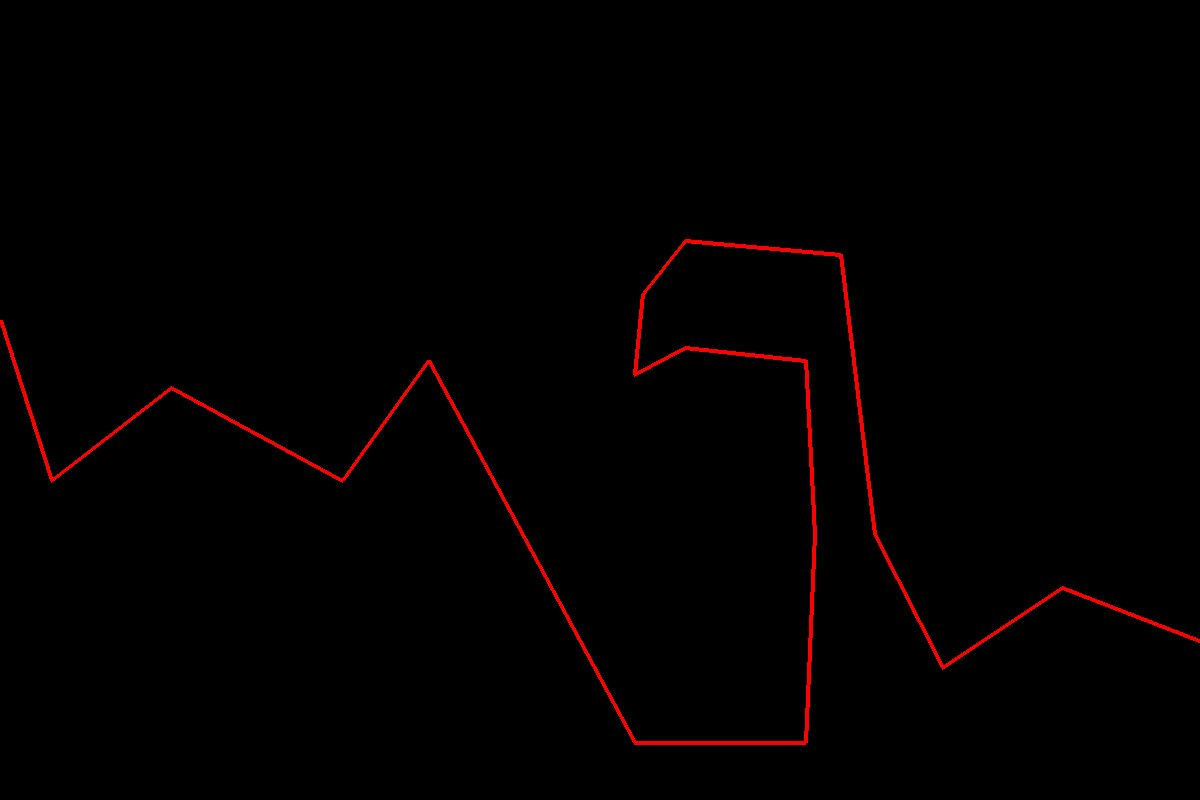
\includegraphics[scale=0.2]{images/cave_map.jpeg}
    \caption{Exemple de carte du problème}\label{fig:map}
\end{figure}

\subsubsection{Espace des Etats}

L'état du vaisseau est représenté par un vecteur de 7 valeurs:
\begin{itemize}
    \item $x$: position horizontale
    \item $y$: position verticale
    \item $hSpeed$: vitesse horizontale
    \item $vSpeed$: vitesse verticale
    \item $fuel$: quantité de carburant restante
    \item $rotate$: angle de rotation
    \item $power$: puissance des moteurs
\end{itemize}
Certains de ces paramètres est borné par une valeur minimale et maximale que voici: 

\begin{itemize}
    \item $x$: $[0, 7000]$
    \item $y$: $[0, 3000]$
    \item $fuel$: $ [0, \infty [ $ 
    \item $rotate$: $[-90, 90]$
    \item $power$: $[0, 4]$
\end{itemize}

\subsubsection{Espace des Actions}

Toutes les secondes, en fonction des paramètres d’entrée (position, vitesse, fuel, etc.), 
le programme doit fournir le nouvel angle de rotation souhaité ainsi que la nouvelle puissance des fusées de Mars Lander.
Mais les commandes de puissance des fusées et de l’angle de rotation sont bornés par les valeurs suivantes qui forme l'espace des actions:
\begin{itemize}
    \item rotation: $[-15, 15]$ 
    \item puissance: $[-1, 1]$
\end{itemize}

\subsubsection{Conditions d'atterrissage}

Les conditions d'atterissage doivent être représentées:
\begin{itemize}
    \item atterrir sur un terrain plat
    \item atterrir en position verticale (angle d'inclinaison = 0°)
    \item la vitesse verticale doit être limitée ($\le 40m.s^{-1}$ en valeur absolue)
    \item la vitesse horizontale doit être limitée ($\le 20m.s^{-1}$ en valeur absolue)
\end{itemize}

\subsection{Algorithme Génétique}

Afin de résoudre ce problème, nous avons choisi d'utiliser une approche heuristique, les algorithmes génétiques.

Les algorithmes génétiques sont des algorithmes d'optimisation stochastique inspirés de la théorie de l'évolution naturelle.
Ils sont basés sur le principe de \textbf{sélection naturelle}.\\
Dans un premier temps on génère une \textbf{population} de solution aléatoire, puis on évalue la qualité de chaque solution.
On sélectionne fait ensuite évoluer cette population à travers des phénomènes semblables à la sélection naturelle tel que la \textbf{sélection}, la \textbf{reproduction} et la \textbf{mutation}.
On répète ce processus jusqu'à ce qu'une solution satisfaisante soit trouvée.
Dans notre problème, une solution est définie par une trajectoire, c'est à dire une suite de commande à effectuer par le vaisseau.\\

\begin{figure}[h]
    \centering
    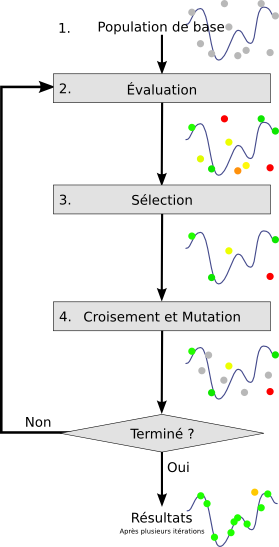
\includegraphics[scale=0.5]{images/schema_simple_algorithme_genetique.png}
    \caption{\cite[]{schema_genetic_algorithm_image}}\label{fig:genetic_algorithm}
\end{figure}

Le calcul du score peut dépendre de nombreux paramètres, dans notre cas on a choisi de prendre en compte les paramètres suivants:
\begin{itemize}
    \item La \textbf{distance} au sol qui sépare la zone de collision et d'atterissage
    \item Les \textbf{vitesses} verticale et horizontale 
    \item L'\textbf{angle} d'inclinaison du vaisseau à l'atterissage
\end{itemize}


\subsection{Objectif}

Afin de bien étudier le problème et l'influence des hyperparamètres de la solution , nous avons décidé de créer une interface graphique.
Pour cela on à définit plusieurs points afin de mener à bien notre projet: 
\begin{itemize}
    \item Création d'une \textbf{interface graphique} sur pygame
    \item Mise en place d'une \textbf{interface client} permettant de piloter la navette
    \item Calcul de \textbf{solution} notamment à l'aide d'algorithme génétique    
\end{itemize}

\subsubsection{Cahier des charges}

Développer une applicattion avec interface graphique. Les fonctionnalités attendues sur l'application sont les suivantes:
\begin{itemize}
    \item Choix de la solution à utiliser
    \item Choix de la carte à utiliser
    \item Exécution de la simulation
    \item Adapter l'affichage en fonction de la solution
\end{itemize}

\subsection{Organisation du projet}

\subsubsection{Répartition des tâches}

En claire la répartition des tâches est la suivante:
\begin{itemize}
    \item \textbf{Augustin Bresset}\\
        Développement de l'environnement et des solutions 
    \item \textbf{Zacharie March}\\
        Développement de l'interface graphique et de l'interface client
\end{itemize}
Dans les deux cas, un apprentissage de la librairie pygame est nécessaire. Que ce soit pour la création de la solution "manuelle" (contrôle par l'utilisateur)
ou pour la création de l'interface graphique.

\subsubsection{Outils de travail}

Afin de communiquer, nous nous reposons pour la communication active sur plusieurs outils, étant deux,
nous n'étions pas restreint par le besoin de créer un groupe sur un outil de communication.
Pour la commun passive nous avons créée une organization sur Github dans laquelle on peut trouver deux repertoire:
\begin{itemize}
    \item \textbf{backend}: Contient le code source du projet
    \item \textbf{meta}: Contient la documentation du projet (et ce livrable)
\end{itemize}

\subsubsection{Organisation du code}

Afin de faciliter la lecture du code ainsi que le développement, nous avons séparer en plusieurs modules le code source:
\begin{itemize}
    \item \textbf{environment}: Contient le code source de l'environnement
    \item \textbf{gui}: Contient le code source de l'interface graphique
    \item \textbf{solution}: Contient le code source des solutions
    \item \textbf{utils}: Contient le code source des fonctions utilitaires
\end{itemize}



\section{Développement}

\subsection{Architecture du projet}

Afin de mener notre projet à bien, nous avons décidé de découper le code en plusieurs modules.
\begin{figure}[h]
    \centering
    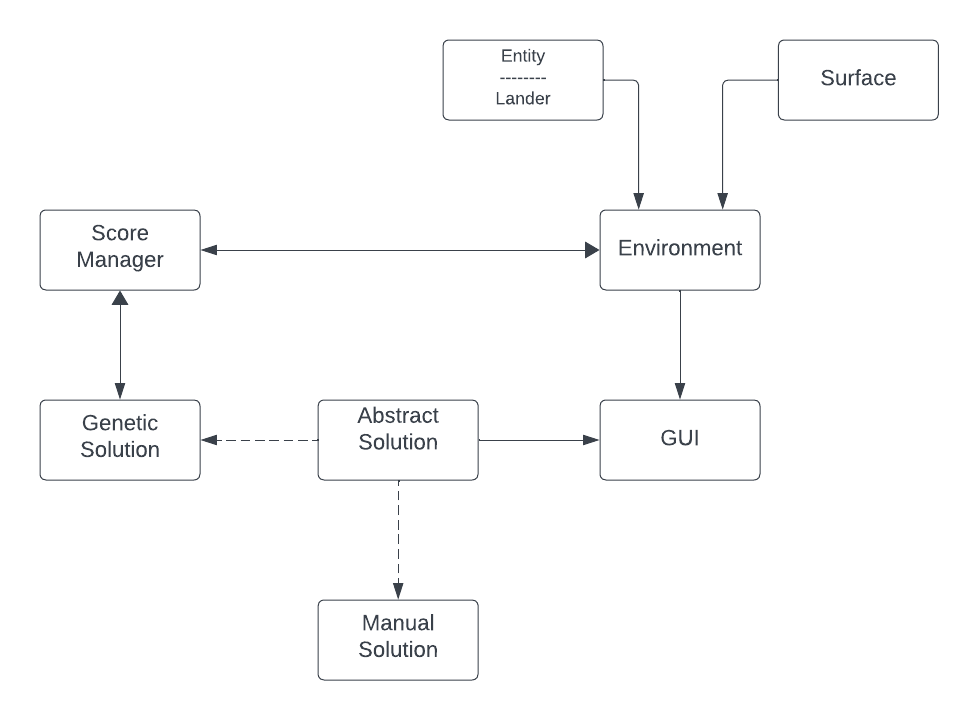
\includegraphics[scale=0.5]{images/class_diagram.png}
    \caption{Architecture du projet}\label{fig:architecture}

\end{figure}


Comme vue dans la figure \ref{fig:architecture}, le projet est composé de plusieurs modules:
\begin{itemize}
    \item \textbf{Environment}: Module permettant de gérer l'environnement
    \item \textbf{Gui}: Module permettant de gérer l'interface graphique
    \item \textbf{Solution}: Module permettant de gérer les solutions
    \item \textbf{Score}: Module permettant de gérer le scoring
\end{itemize}
Et à cela s'ajoute un module \textbf{Utils} qui contient des fonctions utilitaires.

\subsubsection{Environnement}

L'environnement est composé de plusieurs classes:
\begin{itemize}
    \item \textbf{Environment}: Objet permettant de gérer les interactions entre les entités et l'environnement
    \item \textbf{Surface}: Classe permettant de gérer la surface de Mars
    \item \textbf{Lander}: Classe permettant de gérer le vaisseau
    \item \textbf{Action}: Classe permettant de gérer les actions du vaisseau
    \item \textbf{Utils}: Ensemble de fonctions utilitaires et constantes 
    \item \textbf{Entity}: Classe abstraite permettant de gérer les entités
    \item \textbf{Constants}: Classe permettant de gérer les constantes
\end{itemize}


\subsubsection{Gui}
\begin{itemize}
    \item \textbf{Gui}: Classe permettant de gérer l'interface graphique
    \item \textbf{Menue}: Fonction permettant l'affichage du menue
    \item \textbf{Utils}: Ensemble de fonctions utilitaires et constantes
\end{itemize}

\subsubsection{Solution}    

Une solution est définie par une classe abstraite \textbf{AbstractSolution} qui permet de définir les méthodes communes à toutes les solutions.
On a ensuite deux types de solutions:
\begin{itemize}
    \item \textbf{ManualSolution}: Solution manuelle permettant de piloter le vaisseau à l'aide du clavier
    \item \textbf{GeneticSolution}: Solution génétique permettant de piloter le vaisseau à l'aide d'un algorithme génétique
\end{itemize}

\subsubsection{Score}

Le score est calculé à l'aide de la classe \textbf{ScoreManager} qui permet d'attribuer un score à une trajectoire. 
Pour cela il va venir calculer différents résultats sur l'environnement avant qu'il ne soit réinitialisé avant une prochaine simulation.


\subsubsection{Utils}

Le module \textbf{Utils} contient des fonctions utilitaires et des constantes utilisées dans les autres modules et notamment les classes
\textbf{Point} et \textbf{Segment}.

\textbf{Point}\\
La classe Point permet de représenter un point dans un espace à deux dimensions. Il lui ait associé des fonctions permettant de calculer la distance et de gérer
les égalités entre deux points. 
On a considérer ici que deux points étaient égaux si leurs coordonnées étaient assez proches.

\textbf{Segment}\\
La classe Segment permet de représenter un segment dans un espace à deux dimensions.
Sa méthode la plus utile est la méthode \textbf{collision} qui à l'aide d´une fonction \cite[CCW]{ccw_intersect_detection} permet de savoir si deux segments se croisent.

En considérant un instant de trajectoire comme étant un segment, on peut vérifier si il ne rentre pas en collision avec la surface grâce à cette méthode.

\subsection{Tests}

Afin de vérifier le bon fonctionnement de notre code, nous avons mis en place des tests.
Ces tests se divisent en trois catégorites qui composent ces parties.
On va voir dans un premier temps les \textbf{tests unitaires} qui permettent de tester les fonctions et méthodes importantes et de manières indépendantes
au reste du code.
Il enn suivra les \textbf{tests d'intégration} qui permettent de tester le bon fonctionnement des modules entre eux.
Et enfin les \textbf{tests fonctionnels} qui permettent de tester le bon fonctionnement de l'application dans son ensemble.

Nous utiliserons la librairie \textbf{unittest} pour l'écriture de nos tests.

\subsubsection{Tests unitaires}

\textbf{Environnement}
Afin de tester l'environnement, nous avons récuperer les réponses dynimiques de l'environnement présent sur \cite[CodinGame]{codingame_mars_lander} 
et nous avons comparer les états à chaque instant à ceux calculer par notre environnement.\\
De plus on a fait des tests pour vérifier que les collisions avec la surface étaient bien détectées. 
Et notamment que les collisions avec avec le site d'atterissage est bien détecté et que si le vaisseau 
sort de la carte, ce soit bien détecté par l'environnement.


\textbf{Score}
Les fonctions étant simplement des fonctions mathématiques dépendant d'un paramètre du problème, nous n'avons pas jugé nécessaire de faire des tests unitaires
excepté pour la fonction qui permet de calculer la distance entre la zone de collision et la zone d'atterissage.
En effet, ce n'est pas une simple distance euclidienne, mais plutot la distance en suivant la surface de l'environnement.
On a pu vérifier le bon fonctionnement de cette fonction à l'aide de cas caculé à la main.
Et les trois tests nous permettent de nous laisser penser que :
\begin{itemize}
    \item La distance est bien décroissante si l'on se dirige vers la zone d'atterissage
    \item La distance est bien calculée
\end{itemize}

\textbf{Algorithme Génétique}
Ces tests unitaires sont destinés à évaluer le fonctionnement de certaines fonctionnalités de l'algorithme génétique mise en œuvre.

On test tout d'abord la génération d'une population. Il crée une population de 10 individus, chacun ayant 100 gènes du type "ActionChromosome". 
Les assertions comparent la longueur de la population, la longueur des gènes du premier individu, 
et s'assurent que la longueur des gènes est la même pour tous les individus, tout en vérifiant qu'il y a des différences entre les gènes des deux premiers individus.
    
Puis on test la \textbf{cumulative wheel}, ce test évalue la fonction qui génère une roue cumulative pour la sélection d'individus. 
Une population de 10 individus est créée avec des scores aléatoires. 
La population est triée en fonction des scores, puis la roue cumulative est générée. 
Les assertions vérifient que la longueur de la roue cumulative est correcte, 
et que chaque élément de la roue est une paire d'individus de type "ActionChromosome", avec des identifiants différents.

Enfin on vérifie \textbf{la sélection} du/des meilleur individu dans une population.Ce test évalue la fonction de sélection du meilleur individu dans une population. 
Une population de 10 individus est créée, chaque individu ayant un score égal à son index. La population est triée en fonction des scores,
et la meilleure solution est sélectionnée. Les assertions comparent le score de la meilleure solution avec l'index attendu, soit 9 dans ce cas.
En résumé, ces tests garantissent le bon fonctionnement de différentes parties de la solution génétique, y compris la génération de populations, la création de roues cumulatives pour la sélection, et la sélection du meilleur individu dans une population.

\subsection{Problèmes rencontrés}

Tout au long du projet, on a essayé de garder une architecture de code permettant une meilleure répartition des processus
tout en gardant une cohérence dans le code. 

Nous voulions diviser les repertoires github entre le frontend et le backend, mais nous avons finalement pas rencontrés ce besoins étant donné
que l'on travaillait sur le même langage. 

N'ayant pas de deadline claire, on a pu prendre le temps de bien réfléchir à l'architecture du code et à la répartition des tâches mais 
ca nous a aussi conduit a prendre plus de temps que nécessaire pour certaines tâches.
Finalement, on s'est remis à faire des deadlines pour pouvoir avancer plus rapidement.



\subsection{Manuel utilisateur}

Afin de lancer le programme, il faut tout d'abord installer les dépendances du projet présentes dans le fichier \textbf{requirements.txt}.
Pour cela on peut utiliser la commande suivante:
\begin{lstlisting}[style=bash]
    pip install -r requirements.txt
\end{lstlisting}


Une fois les dépendances installées, on peut lancer le programme à l'aide de la commande suivante:
\begin{lstlisting}[style=bash]
    python src/launcher.py
\end{lstlisting}


\printbibliography
\end{document}
